\documentclass[10pt]{article}
\usepackage[spanish]{babel}
\selectlanguage{spanish}
\usepackage[utf8]{inputenc}
\usepackage{graphicx}
\usepackage[lmargin=3cm,rmargin=3cm,tmargin=3cm,bmargin=3cm]{geometry}
\usepackage{amsmath}
\usepackage{amsfonts}
\usepackage{amssymb}
\title{Tiro parabólico con fricción}
\author{Luisa Fernanda Orci Fernandez.}
\date{20 de Abril del 2015}


\begin{document}

\maketitle

\section{Tiro parabólico con fricción en FORTRAN}
En ésta practica diseñamos un programa en FORTRAN que calcule la posición de un objeto que es lanzado mediante un tiro parabólico. Utilizimos como referencia la actividad anterior, solo que ahora consideramos la fricción del aire y comparamos ambos casos.

Las formulas que se toman en cuenta cuando no hay fricción son sencillas, ya que solo actua el peso y la aceleración en el eje $ x $ será cero, y en el eje $ y $ la aceleración es la gravedad. Pero al considerar la fricción, esto cambia. 

Primero tomamos en cuenta que la fricción $ f $ es mas o menos proporcional al cuadrado de la velocidad de nuestro proyectil, $ f = Dv^2 $, donde $ v^2 = v_x^2 + v_y^2 $. La dirección de $ f $ es opuesta a la de la velocidad, entonces $ f = -Dv^2 $, descomponiendo en componente $ x $ y $ y $: $$ f_x = -Dvv_x $$ y $$ f_y = -Dvv_y $$

Considerando la segunda ley de Newton la formulas para calcular la aceleración en $ x $ y $ y $ serán: 

$$ a_x = -(D/m)vv_x $$
$$ a_y = -g-(D/m)vv_y $$

La constante $D$ se calcula con la densidad del aire, el área y el coeficiente de fricción del proyectil: 
$$ D = \frac{\rho(CA)}{2} $$

La formula para calcular la posición en $ x $ del proyectil es:

$$ x+\Delta(x) = x+v_x\Delta(t)+\frac{1}{2}a_x(\Delta(t))^2 $$

y en $ y $:

$$ y+\Delta(y) = y+v_y\Delta(t)+\frac{1}{2}a_y(\Delta(t))^2 $$

\newpage

\subsection{Código}
El código utilizado para crear el programa fue el siguiente:

\begin{verbatim}
module constantes1

implicit none

   real , parameter :: pi = 3.14159265359
   real , parameter :: radianes = (pi)/180

   integer , parameter :: puntos = 5000, muestreo = 1000

   real , parameter :: densidad = 1.18, gravedad = 9.81
   real , parameter :: CoefEsfera = 0.47

end module constantes1

program proyectil

use constantes1

implicit none

real :: xInicial, yInicial, velocidadInicial, anguloInicial 
real :: xMax, yMax, tiempoFinal
real :: xMaxF, yMaxF, tiempoFinalF
real :: diferencia
integer :: ret

write (*,*) 'Introduzca la posicion inicial de tiro en "x" y "y"'
read * , xInicial
read * , yInicial
write (*,*) 'Introduzca la velocidad inicial del proyectil en m/s'
read * , velocidadInicial

write (*,*) 'Introduzca el angulo inicial en grados'
read * , anguloInicial

anguloInicial = anguloInicial*radianes


 
call no_friccion (xInicial, yInicial, velocidadInicial, anguloInicial, xMax, yMax, tiempoFinal)
call si_friccion (xInicial, yInicial, velocidadInicial, anguloInicial, xMaxF, yMaxF, tiempoFinalF)

diferencia = (((xMax-xMaxF)/xMax)*100)


Print * , "------------------------------------------------------------"
Print * , "SIN FRICCION"

Print * , "Posicion inicial del tiro en x=", xInicial, "y=", yInicial
Print * , "Con velocidad inicial de:", velocidadInicial , "m/s"
Print * , "Y un angulo inicial de:", anguloInicial , "radianes"
Print * , "Distancia horizontal maxima =", xMax, "m, y vertical = ", yMax,"m"
Print * , "Tiempo de vuelo de ", tiempoFinal, "s"

Print * , "------------------------------------------------------------"
Print * , "CON FRICCION"
Print * , "Posicion inicial del tiro en x=", xInicial, "y=", yInicial
Print * , "Con velocidad inicial de:", velocidadInicial , "m/s"
Print * , "Y un angulo inicial de:", anguloInicial , "radianes"
Print * , "Distancia horizontal maxima =", xMaxF, "m, y vertical =", yMaxF, "m"
Print * , "Tiempo de vuelo de " , tiempoFinalF, "s"

Print * , "La diferencia es de ", diferencia, "%"

ret = SYSTEM('gnuplot graph.txt')

endprogram proyectil




subroutine no_friccion (xInicial, yInicial, velocidadInicial, anguloInicial, xMax, yMax, tiempoVuelo)

use constantes1
implicit none

integer :: i
Real :: xInicial, yInicial, velocidadInicial, anguloInicial
Real :: xMax, yMax, tiempoVuelo, incrementoTiempo, tiempo
real :: xact, yact, vx, vy

xMax = xInicial + ((velocidadInicial*velocidadInicial+sin(2*anguloInicial))/(gravedad))
yMax = yInicial + (((velocidadInicial*velocidadInicial)*(sin(anguloInicial)*sin(anguloInicial)))/(2*gravedad))
tiempoVuelo = (2*velocidadInicial*sin(anguloInicial))/(gravedad)
incrementoTiempo = tiempoVuelo/muestreo

open (1, FILE = "no_friccion.dat")

!Calcular las velocidad
   vx=(velocidadInicial)*(cos(anguloInicial))
   if (vx < 0) then
      vx = -1*vx
   end if
   vy=(velocidadInicial)*(sin(anguloInicial))


tiempo = 0.0
do i = 1, muestreo

    xact = xInicial + (vx*tiempo)
    yact = yInicial + (vy*tiempo) - (0.5*gravedad*tiempo*tiempo)

    write(1,*) xact, yact
	
    tiempo = tiempo + incrementoTiempo

end do


endsubroutine



subroutine si_friccion (xInicial, yInicial, velocidadInicial, anguloInicial, xMaxF, yMaxF, tiempoVueloF)

use constantes1

implicit none 

integer :: i 

real, dimension (0:muestreo) :: x, y, tiempo, velx, vely, aceleracionX, aceleracionY
real :: xInicial, yInicial, velocidadInicial, anguloInicial
real :: xMaxF, yMaxF, tiempoVueloF
real :: L, area, radio, masa
real, parameter :: deltaT = 0.01

print * , "Introduzca la masa de la esfera en kg"
read * , masa

print * , "Introduzca el radio de la esfera en m"
read *, radio

area = pi*radio*radio

x(0) = xInicial
y(0) = yInicial

velx(0) = velocidadInicial*cos(anguloInicial)
vely(0) = velocidadInicial*sin(anguloInicial)

L = (0.5*densidad*area*CoefEsfera)


aceleracionX(0) = -(L/masa)*(sqrt((velx(0)*velx(0)) + (vely(0)*vely(0)))*velx(0))
aceleracionY(0) = -gravedad-(L/masa)*(sqrt((velx(0)*velx(0)) + (vely(0)*vely(0))))*vely(0)

tiempo(0) = 0

open (2, file = "si_friccion.dat")

write(2,*) x(0), y(0)

do i = 0, muestreo
    tiempo(i+1) = tiempo(i) + deltaT

    velx(i+1) = velx(i) + aceleracionX(i)*tiempo(i+1)
    vely(i+1) = vely(i) + aceleracionY(i)*tiempo(i+1)

    aceleracionX(i+1) = -(L/masa)*(sqrt((velx(i)*velx(i))+(vely(i)+vely(i))))*velx(i)
    aceleracionY(i+1) =  -gravedad-(L/masa)*(sqrt((velx(i)*velx(i))+(vely(i)+vely(i))))*vely(i)

    x(i+1) = x(i)+velx(i)*tiempo(i+1)+(0.5*aceleracionX(i)*tiempo(i+1)*tiempo(i+1))
    y(i+1) = y(i)+vely(i)*tiempo(i+1)+(0.5*aceleracionY(i)*tiempo(i+1)*tiempo(i+1))

    write (2,*) x(i+1), y(i+1)

    if (y(i+1)<0) then
        exit
    end if
end do

close (2)
xMaxF = x(i)
yMaxF = MAXVAL(y)
tiempoVueloF = tiempo(i)*10.0

end subroutine si_friccion
\end{verbatim}

\newpage

\subsection{Resultados}
Aquí un ejemplo final de como quedo el program.

\subsubsection{30 grados}

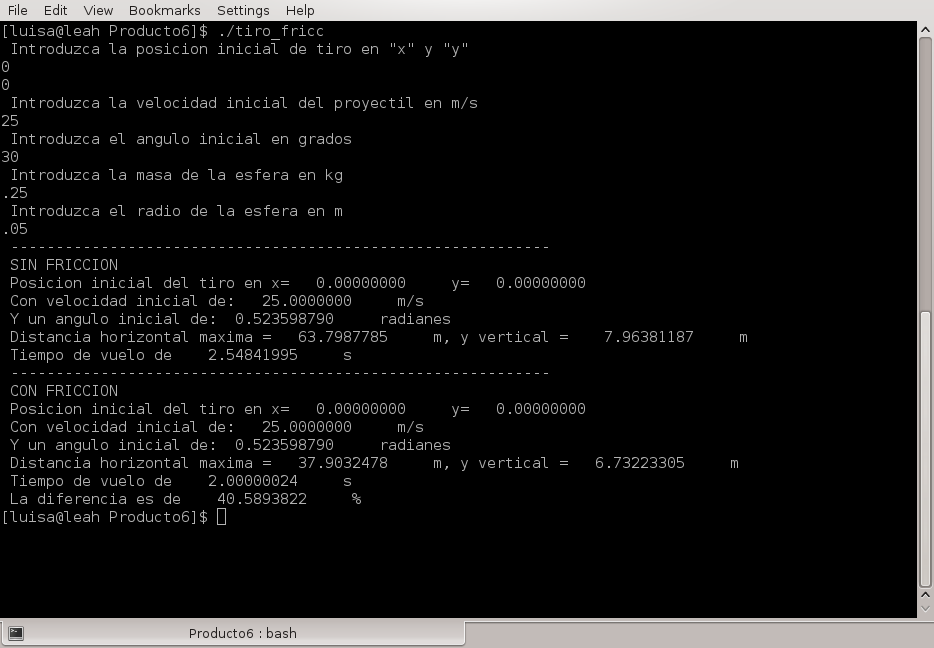
\includegraphics[scale=0.6]{30grad.png}
\\
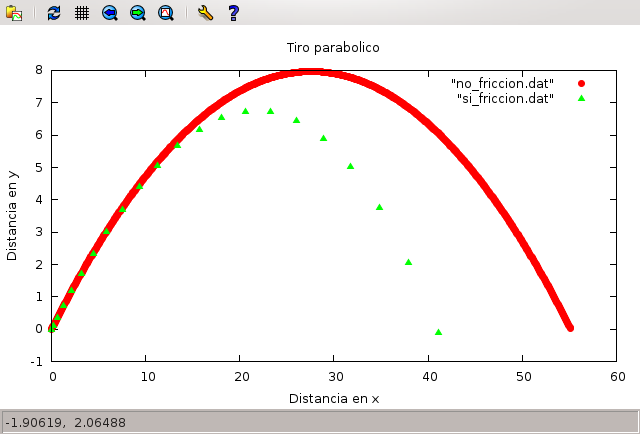
\includegraphics[scale=0.6]{30graf.png}

\newpage

\subsubsection{60 grados}

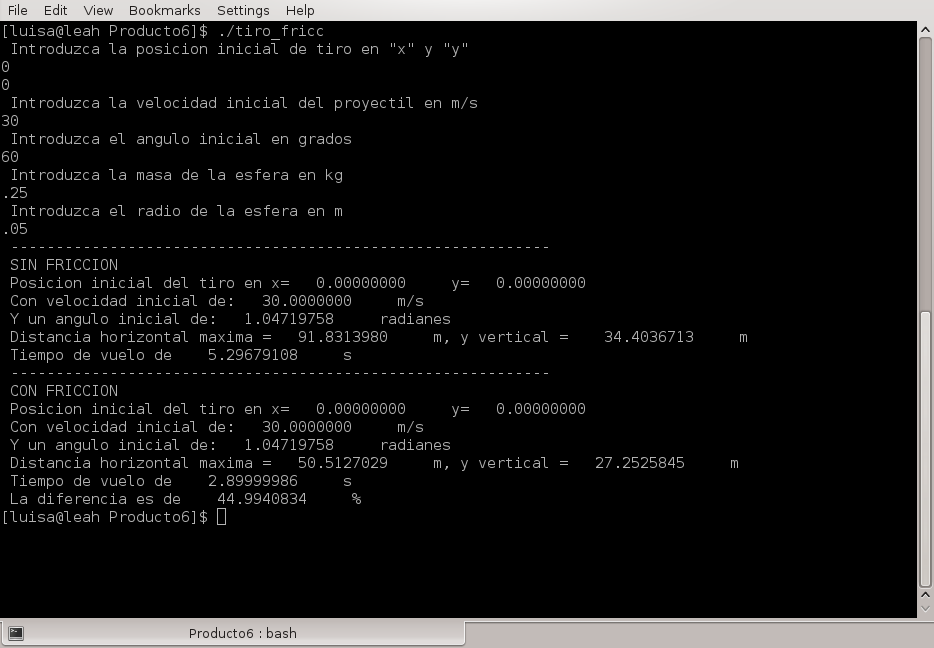
\includegraphics[scale=0.6]{60grad.png}
\\
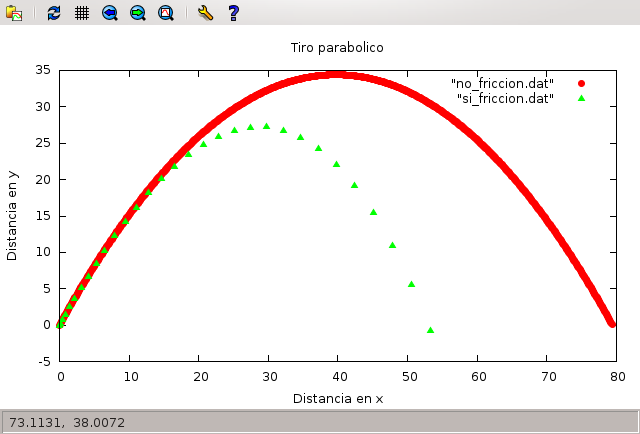
\includegraphics[scale=0.6]{60graf.png}

\newpage

\subsubsection{45 grados}

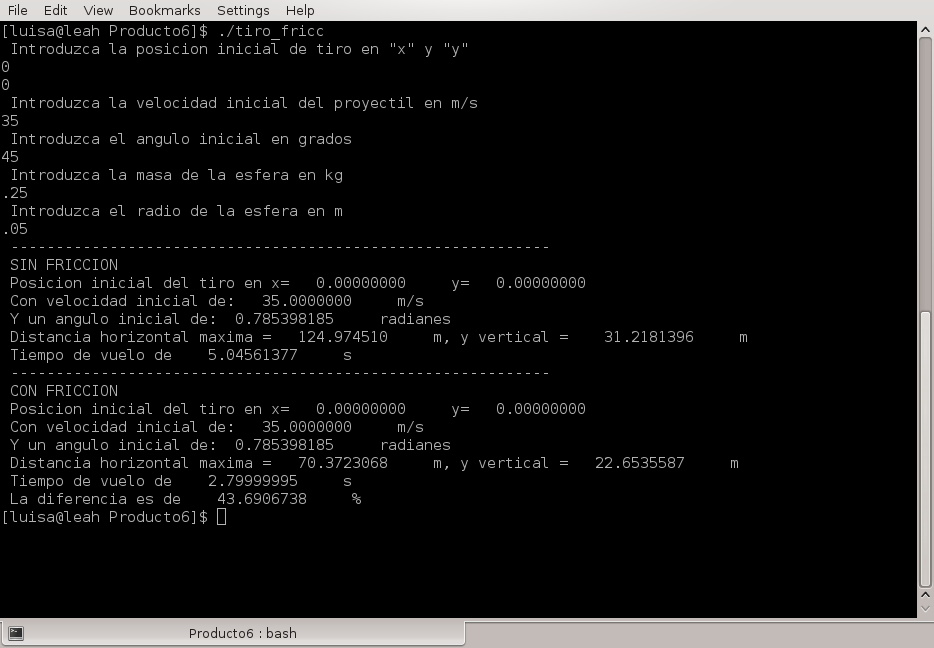
\includegraphics[scale=0.6]{45grad.png}
\\
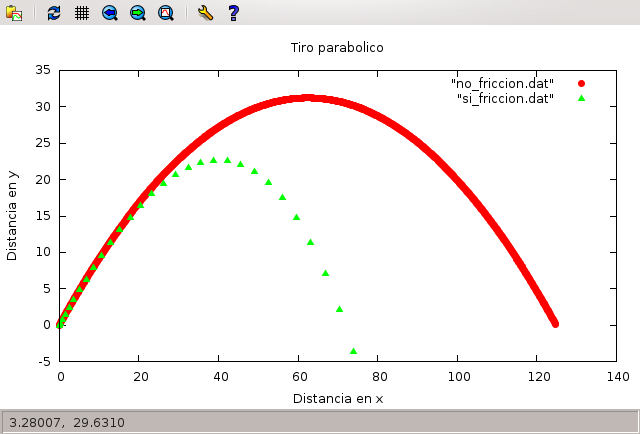
\includegraphics[scale=0.6]{45graf.png}


\end{document}
